\section{Kubo Formula}
We'll derive the Kubo formula for a general, multi-particle (or, if you prefer, single particle) Hamiltonian $H_0$ where the subscript 0 means that this is the unperturbed Hamiltonian before we apply an electric field. We denote the eigentstates of the Hamiltonian as $\ket m$ with $H_0\ket m=E_m \ket m$.
\begin{equation}
    H_0=\sum_i\left[\frac{1}{2m}\left(\vect p_i-e\vect A_0\right)^2 + V_0(\vect r_i)\right]+\sum_{i\neq j}V_{ee}(\vect r_i-\vect r_j)
\end{equation}
Where $\vect A_0$ and $V_0$ are due to an existing EM field. Now we add a background electric field. We 
\begin{equation}
    H=\sum_i\left[\frac{1}{2m}\left(\vect p_i-e\vect A_0 - e\vect A\right)^2 + V_0(\vect r_i) - e\vect r_i\phi(\vect r_i)\right]+\sum_{i\neq j}V_{ee}(\vect r_i-\vect r_j)
\end{equation}
Which can be written as 
\begin{equation}
    H=H_0 + \sum_{i}-\frac{e}m \boldsymbol \pi_i\cdot \vect A - e\vect r_i\phi(\vect r_i)
    \label{eq:temp_ham}
\end{equation}
Where $\boldsymbol \pi_i=\vect p -e\vect A_0=m\dot{\vect r}$ is the mechanical momentum,
furthermore we can use the fact that the electric charge operator $\rho(\vect r)=-e\sum_{i}\delta(\vect r-\vect r_i)$ current operator  $\vect I$ is equal to 
\begin{equation}
    \vect I=-e\sum_{i}\dot{\vect r}_i=-\sum_{i}\frac{e}m \boldsymbol \pi_i
\end{equation}
to re-write equation \ref{eq:temp_ham} like so
\begin{equation}
    H=H_0+\vect I\cdot \vect A + \int\rho(\vect r)\phi(\vect r)d\vect r
\end{equation}
however, we can assume that the density of charge $\rho$ is always zero (it is usually considered when investigating dielectric properties of a material, but here we are interested in conduction, so we are ignoring it)
\begin{equation}
    H(\vect A)=H_0+\vect I\cdot \vect A
    \label{eq:deltaH}
\end{equation}
At this point we need to write the perturbation in terms of the electric field, we can choose a gauge where $\vect E=-\partial_t\vect A$ and assume that the wave is monochromatic $\vect E(t)=\vect Ee^{-i\omega t}$, so 
\begin{equation}
    A=\frac{ \vect E}{i\omega}e^{i\omega t}
    \label{eq:A(E)}
\end{equation}
Our goal is to compute the current $\langle \vect I\rangle$ that flows due to the perturbation $\Delta H$. To do so we'll work in the \textit{interaction picture}, this means that the operators evolve as $\mathcal O(t)=V^{-1}\mathcal O V$ with $V=e^{-iH_0t/\hbar}$. This means that the states evolve by 
\begin{equation}
    \ket{\psi(t)}=U(t,t_0)\ket{\psi(t_0)}; \quad 
    U(t,t_0)=T\exp\left(-\frac i\hbar \int_{t_0}^t\Delta H(t')dt'\right)
    \label{eq:int evol}
\end{equation}
Where $T$ is the time ordering, keep in mind that since we are in the interaction picture $\Delta H(t)=V^{-1}\Delta HV$.\\
We now prepare the system at time $t=-\infty$ in a specific many body state $\rho_0=\sum_i p_i\ket{i}\bra{i}$ (it usually is either the ground state or a thermodynamic distribution). Keep in mind that the density operator, in the interaction picture evolves with the states
\begin{equation}
\begin{split}
        \rho(t)&=\sum_ip_i\ket{\psi_i(t)}\bra{\psi_i(t)}=\\
        &0=\sum_ip_iU(t,t_0)\ket{\psi_i(t_0)}\bra{\psi_i(t_0)}U^{-1}(t,t_0)=\\
        &=U(t,t_0)\rho(t_0)U^{-1}(t,t_0)
\end{split}
\end{equation}
Then, writing $U(t)=T(t,t_0\to-\infty)$, the expectation value of the current is
\begin{equation}
    \begin{split}
        \langle \vect I(t)\rangle &= \tr\left[\rho(t)\vect I(t)\right]=\\
        &=\tr\left[U(t)\rho_0 U^{-1}(t) \vect I(t)\right]=\\
        &=\tr\left[\rho_0 U^{-1}(t) \vect I(t)U(t)\right]=\\
        &=\langle U^{-1}(t) \vect I(t)U(t)\rangle_{0}\approx\\
        &\approx\left\langle\vect I(t)\right\rangle_{0} +
        \left\langle \frac i\hbar \int_{-\infty}^t[\Delta H(t'),\vect I(t)]dt'\right\rangle_0
    \end{split}
\end{equation}
Where in the last passage we've expanded the exponential in the $U$ operator (equation \ref{eq:int evol}), and $\langle \dots\rangle_0$ means the average with respect to $\rho_0$. The first term is the current in the absence of an electric field, therefore it is zero. Using equation \ref{eq:deltaH} and \ref{eq:A(E)} and plugging it in the last equation we have that the current due to the electric field is then
\begin{equation}
    \langle I_i(t)\rangle=\frac 1{\hbar\omega}\int_{\infty}^t
    \langle[I_j(t'),I_i(t)]\rangle_0 E_je^{-i\omega t'}dt'
\end{equation}
Because the system is invariant under time translations, the correlation function above can bony depend on $t''=t-t'$, we can rewrite the expression above as
\begin{equation}
    \frac{E_je^{-i\omega t}}{\hbar \omega}\int_0^{\infty}e^{i\omega t''} \langle[I_j(0),I_i(t'')]\rangle_0 dt''
\end{equation}.
The only t dependence in the formula above sits outside as $e^{-i\omega t}$. This means that the proportionality constant is the conductance. To get the conductivity $\sigma$ (conductance per unit area, we just have to divide the surface $S$), and the off diagonal part is the \textit{Hall conductivity}
\begin{equation}
    \sigma_{xy}=\frac 1{S\hbar \omega}\int_0^{\infty}e^{i\omega t} \langle[I_x(0),I_y(t)]\rangle_0 dt
    \label{eq:kubo}
\end{equation}
This is the \textit{Kubo formula} for the Hall conductivity.













\section{Quantization of Hall conductivity}
Our job here is not done, we got Kubo formula the Hall conductivity \ref{eq:kubo}, but to capture the most important property we need to do some mathematical manipulation. Using the fact hat $\vect I(t)=V^{-1}\vect I(0) V$ with $V=e^{-iH_0t/\hbar}$ we can write
\[
    \sigma_{xy}(\omega)=\frac 1{S\hbar \omega}\int_0^{\infty}e^{i\omega t}\sum_{nm}p_n
    \left[
        \braket{n|I_y}{m}\braket{m|I_x}{n}e^{-iE_{nm}t/\hbar}-(n\leftrightarrow m) %\braket{n|J_x}{m}\braket{m|J_y}{n}e^{i(E_n-E_m)t/\hbar}
    \right]
    dt
\]
Now we can perform the integral in $dt$, since the states with $n=m$ cancel out we have that
\begin{equation}
    \sigma_{xy}(\omega)=-\frac i{\omega S} \sum_{nm}p_n\left[
        \frac{\braket{n|I_y}{m}\braket{m|I_x}{n}}{\hbar \omega - E_{nm}} - (n\leftrightarrow m)
    \right]
\end{equation}
To get the Hall conductivity for DC current we have to evaluate $\sigma_{xy}(\omega\to 0)$, in this limit
\[
    \lim_{\omega\to 0}\frac{1}{\hbar \omega-E_{nm}}=-\frac 1{E_{nm}}+\frac{\hbar \omega}{(E_{nm})^2}    
\]
Plugging the zeroth-order we get
\begin{equation}
    \begin{split}
    \sigma_{xy}=&\frac i{\omega S} \sum_{nm}p_n\left[
        \frac{\braket{n|I_y}{m}\braket{m|I_x}{n}}{E_{nm}} - (n\leftrightarrow m)
    \right]= \\
    =&\frac i{\omega S}\sum_{nm}\frac{p_n}{E_{nm}}\left[
        \braket{n|I_y}{m}\braket{m|I_x}{n} + (n\leftrightarrow m)
    \right]=\\
    =&0
    \end{split}
\end{equation}
That is equal to zero because the terms inside the summation are asymmetric under the exchange of $(n\leftrightarrow m)$, and we are summing over all the possible $n$ and $m$. For the first order term we have
\begin{equation}
    \sigma_{xy}=\frac{i\hbar}S\sum_{nm}\frac{p_n}{(E_{nm})^2}\left[
        \braket{n|I_y}{m}\braket{m|I_x}{n} - (n\leftrightarrow m)
    \right]
    \label{eq:kkubo}
\end{equation}

From equation \ref{eq:deltaH} we can see that $I_i=\partial H/\partial A_i$, this means that the equation above becomes
\begin{equation}
    \begin{split}
        \sigma_{xy}=&
        \frac{i\hbar}S\sum_{nm}\frac{p_n}{(E_{nm})^2}\left[
        \braket{n|I_y}{m}\braket{m|I_x}{n} - (n\leftrightarrow m)
    \right]=\\
    =&\frac \hbar S\sum_{n}p_n\sum_{m\neq n}\frac{i}{(E_{nm})^2}\left[
    \braket{n\bigg|\frac{\partial H}{\partial A_y}}{m}\braket{m\bigg|\frac{\partial H}{\partial A_x}}{n} - (n\leftrightarrow m)
    \right]=\\
    =&\frac \hbar S\sum_{n}p_n\Omega^n_{A_xA_y}
    \end{split}
\end{equation}
This is a nice formula, however it doesn't explain why $\sigma_{xy}$ is quantized, however if we average over all possible values of $\vect A$, which comes from all the possible value of the fluxes

\begin{equation}
    \begin{split}
        \langle\sigma_{xy}\rangle=&
        \frac{\int \sigma_{xy}d^2\vect A}{\int d^2\vect A}=\\
        =&\left(\frac{S}{\Phi_0^2}\right)\frac \hbar S\sum_np_n\int \Omega^n_{A_xA_y}d^2\vect A =\\
        =&\left(\frac{e^2}{4\pi^2\hbar^2}\right)2\pi\hbar\sum_np_nC_n=\\
        =&\frac{e^2}{2\pi\hbar}\sum_np_nC_n\quad \quad \text{with }C_n\in \mathbb Z
    \end{split}
    \label{eq:quantized sigma}
\end{equation}
Where we have defined the Chern numbers $2\pi C_n=\int \Omega^n_{A_xA_y}d^2\vect A$ and for the Stokes theorem it is a multiple of $1$. The most emblematic passage here is why $\int d^2\vect A=\Phi_0^2/S$.\\

\subsubsection*{$\boldsymbol{\sigma_{xy}}$ at low temperatures}
In equation \ref{eq:quantized sigma} we had a contribution that is the average of $C_n$ over all the states, if we are at low temperature there are two possibilities depending on the treatment we had on the wavefunction
\begin{itemize}
    \item \textbf{Many body interacting wavefunction} For $T\to 0$ we have that it will be at the fundamental state $p_0\to1$ and $p_i\to 0$ for $i\neq 0$, this means that $\sum_np_nC_n\to C_0$, therefore a quantized conductivity quill be observed
    \item \textbf{Non-interacting single particle wavefunctions} For $T\to 0$ the electrons will settle in a Fermi-Dirac distribution, so \[\sum_np_nC_n=N^{-1}\sum_nC_n\theta(E_F-E_n)\] where $N$ is the total number of electrons and $E_F$ is the Fermi energy. Although it's not as easy to prove that is generally quantized due to the $N^{-1}$ factor,\footnote{Even thought we know for sure it must be quantized, because we can always re-parametrize Non-interacting single particle wavefunctions into many body interacting wavefunction} we'll see that it's much easier to calculate the precise value for real world scenarios, and it's going to be the subject of the next section
\end{itemize}



















\section{Berry phase in Bloch bands}
\label{sec:berrybloch}
The band structure of crystals provides a natural platform to investigate the occurrence of the berry phase effect. Within the independent electron approximation, the band structure of a crystal is determined by the Bloch Hamiltonian:
\begin{equation}
    H= \frac {\vect p^2}{2m} + V(\vect r)
\end{equation}
Where $V(\vect r+\vect a)=V(\vect r)$ is the periodic potential with $a$ being the Bravais lattice vector. According to Bloch's theorem the eigenstates satisfy 
\begin{equation}
    \psi_{n\vect k}(\vect r+\vect a)=e^{i\vect k\cdot \vect a}\psi_{n\vect k}(\vect r)
\end{equation}
where $n$ is the band index and $\hbar \vect k$ is the crystal momentum. To comply with the general formalism of the Berry phase, we make the following unitary transformation to obtain a $\vect k$-dependent Hamiltonian

\begin{equation}
    e^{-i\vect k\cdot \vect r}He^{i\vect k\cdot \vect r}\equiv H(\vect k)= \frac {(\vect p+\hbar \vect k)^2}{2m} + V(\vect r)
    \label{eq:k-repr}
\end{equation}
The transformed eigenstate $u_{n\vect k}(\vect r)= e^{-i\vect k\cdot \vect r}\psi_{n\vect k}(\vect r)$ is just the cell-periodic part of the Bloch function. It satisfies the strict periodic boundary condition 
\begin{equation}
    u_{n\vect k}(\vect r+\vect a)=u_{n\vect k}(\vect r)
\end{equation}
We can now identify the Brillouin zone as the parameter space of the transformed Hamiltonian $H(\vect k)$, and $u_{n\vect k}=\ket{n,\vect k}$ as the basis function.\\
In this regime the Kubo formula \ref{eq:kkubo} becomes 
\begin{equation}
    \sigma_{xy}=i\hbar\sum_{m,E_n<E_F}\int_{T^2}
    \frac{
        \braket{n,\vect k|J_y}{m,\vect k}\braket{m,\vect k|J_x}{n,\vect k} - (n\leftrightarrow m)
    }
    {
        E_m(\vect k)-E_n(\vect k)
    }
    \frac{d^2\vect k}{(2\pi)^2}
    \label{eq:tknn}
\end{equation}
And it is called the TKNN formula \cite{thouless1982quantized}

We can define the current in terms of the group velocity of the wavepackets
\begin{equation}
    \vect J=\frac e\hbar \frac{\partial H}{\partial \vect k}
\end{equation}
this means that equation \ref{eq:tknn} is equal to
\begin{equation}
    \sigma_{xy}=\frac{e^2}\hbar \sum_{E_n<E_F}\Omega^n_{k_xk_y}\frac {d^2\vect k}{(2\pi)^2}
    \label{eq:fermi-cond}
\end{equation}
Using the Chern theorem \ref{eq:chern} we have that the equation above is equal to 
\begin{equation}
    \frac{e^2}{2\pi\hbar}\sum_n^N C_n
\end{equation}
where $C_n$ is the Chern number of the $n$-th band and the bands up to the $N$-th band are occupied, therefore we sum over the occupied bands



















\section{Anomalous velocity}
Finally, as a last phenomenon of the Berry curvature we talk about how it changes the velocity of electrons inside crystals. The velocity operator of a particle in a periodic potential with crystal impulse $\vect k$ is given by \cite{grosso2013solid}
\begin{equation}
    \vect v(\vect k)= \frac{\partial H(\vect k)}{\hbar \partial \vect k}
    \label{eq:cryspeed}
\end{equation}
where $H(\vect k)$ is the Hamiltonian from equation \ref{eq:k-repr}. so the velocity of the $n$-th state with impulse $\vect k$ is simply
\begin{equation}
    \vect v_n(\vect k)=\bra{\psi_{n'}}\vect v(\vect k)\ket{\psi_{n'}}=\frac{\partial E_n(\vect k)}{\hbar \partial \vect k}
\end{equation}
Now lets see what happens if we apply a weak uniform external electric field through a uniform vector potential $\vect A(t)$. Using the Peierls substitution, the Hamiltonian is written as 
\begin{equation}
    H(\vect k,t)= \frac{[\vect p+\hbar\vect k +e\vect A(t)]^2}{2m}+V(\vect r)
\end{equation}
we can now introduce a gauge invariant crystal momentum $\vect \pi(\vect k, t)=\vect k +e\vect A(t)$ and we can notice that
\begin{equation}
    H(\vect k,t)=H(\vect \pi)
\end{equation}
Since $\vect A (t)$ preserves the translational symmetry, $\vect k$ is still a good quantum number and it is a constant of motion $\dot{\vect k}=0$ it follows from derivating with respect to time this equation $\vect \pi(\vect k, t)=\hbar \vect k +e\vect A(t)$ that
\begin{equation}
   \dot{\vect\pi}=-e \vect E
   \label{eq:pidt}
\end{equation}
To evaluate the velocity we have to use first order perturbation theory \cite{thouless1983quantization}
\begin{equation}
    \ket{\psi'_n}=\ket{\psi_n}+\sum_{n'\neq n}\frac{\braket{\psi_{n'}}{\Delta H|\psi_n}}{E_{n'}-E_n}\ket{\psi_{n'}}
\end{equation}
since in the interaction picture $\Delta H\ket{\psi_n}=-i\hbar\ket{\partial_t\psi_n}$
we have that the equation above becomes
\begin{equation}
    \ket{\psi'_n}=\ket{\psi_n}-i\hbar\sum_{n'\neq n}\frac{\braket{\psi_{n'}}{\partial_t\psi_n}}{E_{n'}-E_n}\ket{\psi_{n'}}
\end{equation}
from equation \ref{eq:cryspeed} we have that the velocity with the new states becomes 
\begin{equation}
    \begin{split}
        \vect v_n(\vect k)=&\bra{\psi'_n}\vect v(\vect k)\ket{\psi'_n}=\\
        =&\bra{\psi_n}\vect v(\vect k)\ket{\psi_n} -i\sum _{n\neq 0}
        \braket{\psi_n\bigg|\frac{\partial H}{\partial \vect k }}{\psi_{n'}}
        \frac{\braket{\psi_{n'}}{\partial_t\psi_n}}{E_{n'}-E_n} - \textrm {c.c.}
    \end{split}
    \label{eq:start-anom}
\end{equation}
from equation \ref{eq:partial H} we can say that
\begin{equation}
    \braket{\psi_n\bigg|\frac{\partial H}{\partial \vect k }}{\psi_{n'}}\frac1{E_{n'}-E_n}=\braket{\partial_{\vect k}\psi_n}{\psi_{n'}}
\end{equation}
and using equation \ref{eq:cryspeed}, equation \ref{eq:start-anom} becomes
\begin{equation}
    \vect v_n(\vect k)=\frac{\partial E_n (k)}{\hbar\partial \vect k} -i
    \sum_{n'\neq n}
    \braket{\partial_{\vect k}\psi_n}{\psi_{n'}}
    \braket{\psi_{n'}}{\partial_t\psi_n}
    -\textrm{c.c.}
\end{equation}
The second term in the equation above is the Berry curvature (equation \ref{eq:berry-curvature2}), so in the end we get that.

\begin{equation}
    \vect v_n(\vect k)=\frac{\partial E_n (k)}{\hbar\partial \vect k} -\Omega^n_{\vect kt}
    \label{eq:afgubaibg}
\end{equation}
Also, since $\frac{\partial}{\partial \vect \pi}=\frac \partial{\hbar\partial \vect k}$ and $\hbar\frac{\partial \vect k}{\partial t}=-e\vect E$ (equation \ref{eq:pidt})
we have that
\[
    \frac{\partial }{\partial t}=-\frac e\hbar \nabla_{\vect k}\cdot \vect E    
\]
Thought some mathematical manipulation it can be shown that parsing the equation above into equation \ref{eq:afgubaibg} we get that  \cite{chang1995berry}

\begin{equation}
    \vect v_n(\vect k)=\frac{\partial E_n (k)}{\hbar\partial \vect k} -\frac e\hbar \vect E\times \vect \Omega^n(\vect k)
    \label{eq:anomalous_velocity}
\end{equation}
Where $\vect \Omega^n(\vect k)$ is the Berry curvature of the $n$-th band 
\begin{equation}
    \vect \Omega^n(\vect k)=i\bra{\nabla_{\vect k}\psi_n}\times \ket{\nabla_{\vect k}\psi_n}      
\end{equation}
From equation \ref{eq:anomalous_velocity} we can see that, in addition to the usual band dispersion contribution of equation \ref{eq:cryspeed}, an extra term previously known as an anomalous velocity contributes to $\vect v_n(\vect k)$. This velocity is transverse to the electric field, and it gives us yet another way of interpreting the Hall effect.













\section{Symmetry considerations for the Berry curvature}
The velocity formula of equation \ref{eq:anomalous_velocity} shows us that, in addition to the band energy, the Berry curvature is required for a complete description of electron dynamics. However, the conventional formula of equation \ref{eq:cryspeed} has had great success describing electronic properties in the past. This suggests us that the Berry curvature term in most cases does not contribute.

The general form of the Berry curvature $\Omega^n(\vect k)$ can be obtained via symmetry analysis. The velocity formula \ref{eq:anomalous_velocity} should be invariant under time reversal and spatial inversion symmetry if the unperturbed system possesses these symmetries to begin with. Under time reversal, $\vect v_n$ and $\vect k$ changes sign while $\vect E$ does not, in that case from \ref{eq:anomalous_velocity} we have that
\begin{equation}
    \Omega^n(-\vect k)=-\Omega(\vect k)\,.
\end{equation}
Under spatial inversion, $\vect v_n$, $\vect k$ and $\vect E$ changes sign, so from equation \ref{eq:anomalous_velocity}
\begin{equation}
    \Omega^n(-\vect k)=\Omega(\vect k)\,.
\end{equation}
\begin{wrapfigure}{r}{.5\textwidth}
    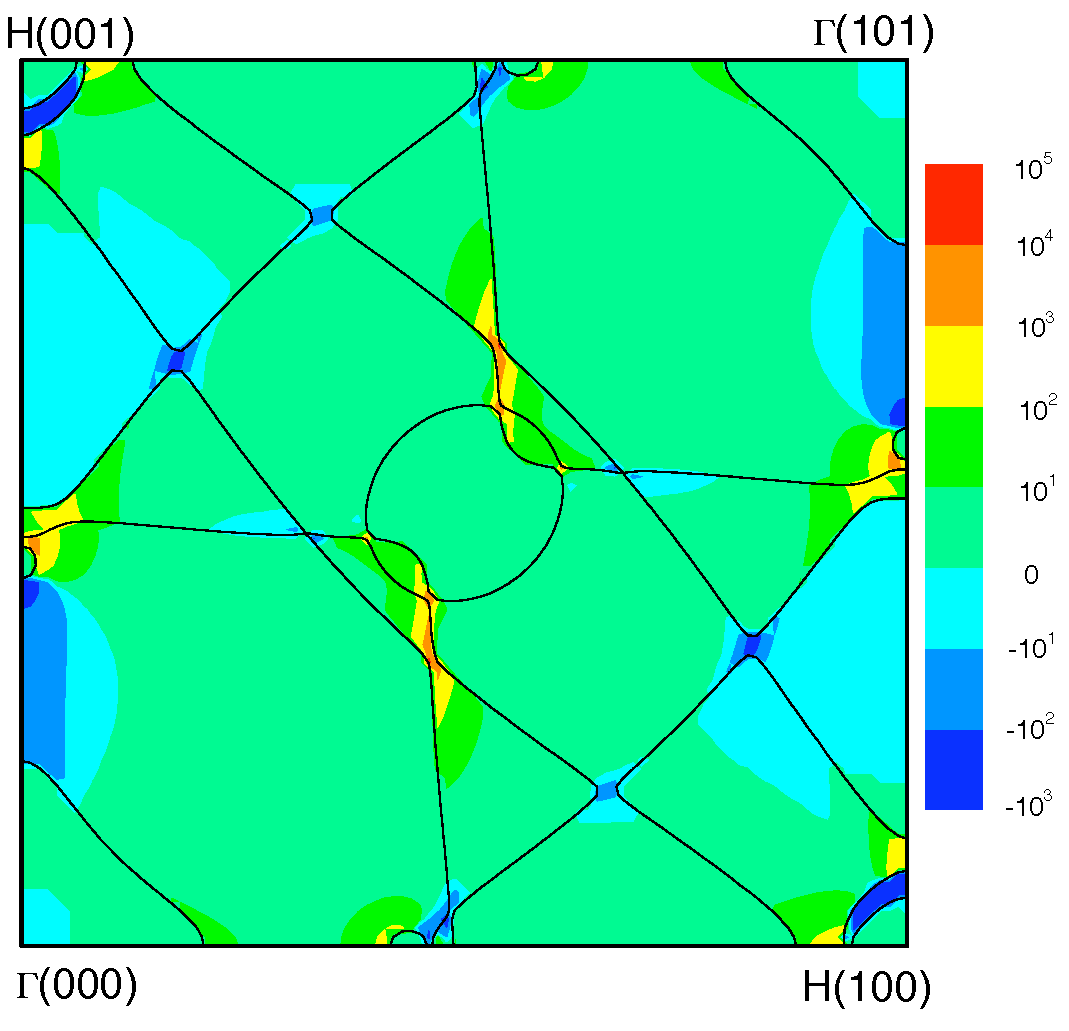
\includegraphics[width=.5\textwidth]{Immagini/topo/curvature_Fe.pdf}
    \caption{This plot represents the intersection of the be Brillouin zone with the 010 plane. The solid line i where the fermi surface intersects the 010 plane and in color in shown the magnitude of the Berry curvature $\Omega_z(\vect k)$ in atomic units \cite{yao2004first}}
    \label{fig:berryferro}
\end{wrapfigure} 
Therefore, fore crystals with simultaneous time-reversal and spatial inversion symmetry the Berry curvature vanish identically throughout the Brillouin zone, this reduces equation \ref{eq:anomalous_velocity} to equation \ref{eq:cryspeed}.


There are many important systems where both symmetries are not simultaneously present, for example in materials where the ferromagnetic ordering breaks the time reversal symmetry (figure \ref{fig:berryferro}).
Another example is provided by single-layered graphene stacked on top of a substrate of Boron nitrite which breaks the inversion symmetry, it will be one of the main focuses of the thesis, but before delving into that we need to talk in more detail about the structure and electronic properties of graphene.

